\section{Värmeflöde genom väggar, burspråk och tak}

\begin{figure}[hpbt]
\centering

\subfloat[\label{fig:tempdistapr}
Utomhustemperaturens variation en dag i april.]{
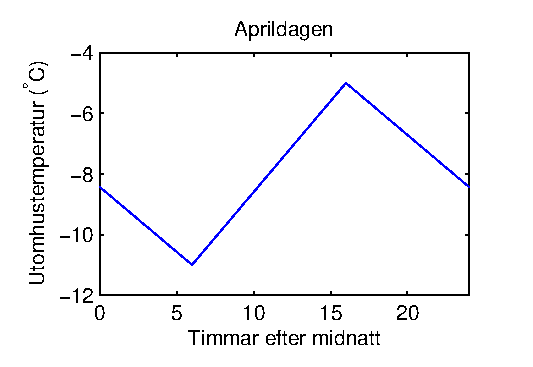
\includegraphics[width=6cm]{images/temperatureapr.eps}}\vspace{1cm}
\subfloat[\label{fig:tempdistdec}
Utomhustemperaturens variation en dag i december.]{
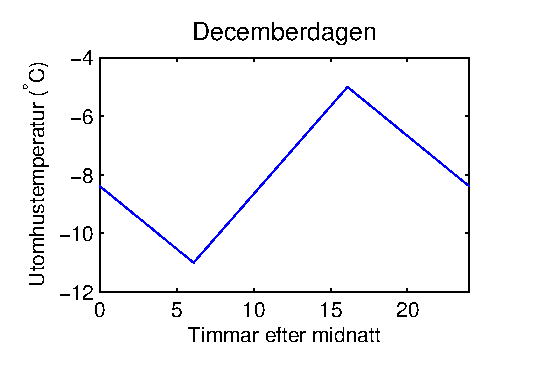
\includegraphics[width=6cm]{images/temperaturedec.eps}
}

\caption{\label{fig:temperaturedist} Utomhustemperaturens variation under standarddagarna motsvarande mitten av april samt den sista december som varierar mellan $\unit[6]{^\circ C}$ på natten och $\unit[9]{^\circ C}$ på dagen respektive $\unit[-11]{^\circ C}$ på natten och $\unit[-5]{^\circ C}$ på dagen.
}
\end{figure}

För att jämföra energiförluster genom en vägg med isolering och utan isolering används
den tidigare beskrivna finita elementmetoden för värmeledningsekvationen i en dimension. Här approximeras
väggen som oändligt lång för simplicitet i beräkningarna. För alla beräkningar så har ett tidssteg
på $\Delta t = \unit[500]{s}$ använts med semidiskret MOL.

I detta försök antags det att en perfekt värmeanläggning
existerar så att temperaturen inomhus hålls till konstanta $\unit[20]{^\circ C}$. Efter detta specificeras energiflödet
från utsidan av väggen genom vilka energiflöden som strömmar till väggen. Dessa är svartkroppsstrålning, solinstrålning
samt konvektion. Beräkningarna är sedan genomförda med solinstrålningsdata från en molning nyårafton,
en solig aprildag samt en molning aprildag. Solens position och mägnden svartkroppsstrålning är beräknade enligt avsnitt
\ref{sec:sunthroughwindows} och avsnitt \ref{sec:blackbody}.
Konvektionsparametern är sedan satt till $h=\unit[6,19]{Wm^{-2}K^{-1}}$ för aprildagen vilket motsvarar en helt vindstilla aprildag.
För decemberdagen sattes konvektionsparametern till $h=\unit{35}{Wm^{-2}K^{-1}}$ vilket motsvarar en decemberdag med en vindhastighet på $v=\unit[7]{ms^{-1}}$ paralellt
med ytan.
Under aprildagen varierade temperaturen linjärt från $T=\unit[6]{^\circ C}$ klockan 06:00 och $T=\unit[9]{^\circ C}$ 16:00 vilket kan ses i figur \ref{fig:tempdistapr}.
Samma värden för decemberdagen är $T = \unit[-11]{^\circ C}$ 06:00 respektive $T=\unit[-5]{^\circ C}$ 16:00 vilket kan ses i figur \ref{fig:tempdistdec}.

Problemet har sedan satts upp för två olika väggar. Först en som enbart innehåller $\unit[5]{dm}$ tegel med
en värmeledningsförmåga på $k = \unit[0.6]{Wm^{-1}K^{-1}}$ och volymetrisk värmekapacitet på
$c_{p}\rho = \unit[1,153846]{MJm^{-3}}$. Den andra väggen har först samma tegellager sedan
har den tilläggsisolerats på utsidan med $\unit[1]{dm}$ mineralull. Denna mineralull har värmeledningsförmåga på
$k = \unit[5,2\cdot 10^{-7}]{Wm^{-1}K^{-1}}$ och volymetrisk värmekapacitet på
$c_{p}\rho = \unit[58,8]{kJ m^{-3}}$. \cite{kandidatarbete2010}\cite{engineeringtoolboxdensity}\cite{bkvthermal}\cite{engineeringtoolboxspecificheat}

Under experimentens gång så har ett godtyckligt initialvärde valts för att sedan vänta tills
lösningen stabiliserat sig för att då urläsa energiåtgången. Derivatan på insidan har slutligen beräknats
och använts för att beräkna kyleffekten genom fouriers värmelag.

För att studera hur de olika väggarna beter sig vid ett stegsvar har ett sådant tillverkats. Experimentet
har startats med att väggarna varit i jämvikt med en utomhustemperatur på $T = \unit[0]{^\circ C}$ för att
sedan stiga till $T = \unit[10]{^\circ C}$ vid tiden $t=0$. Konvektionsparametern är här satt till
$h = \unit[25]{W m^{-2}K^{-1}}$ vilket kommer av en vind på
$v = \unit[5]{ms^{-1}}$ paralellt med väggens yta. Slutligen så kunde väggarnas
tröghet studeras genom att den momentana kyleffekten beräknades för varje tidssteg. 

För burspråk och tak har ungefär samma metod följts som för väggen, med simuleringar motsvarande soliga och
molniga december- respektive aprildagar. Samma temperaturförändringar som beskrivits ovan har använts för
respektive fall. Skillnaden ligger för det första i vilka material de olika byggnadsdelarna är uppbyggda av.
Burspråket har, som i \ref{fig:bursprak}, simulerats med materialen och tjocklekarna angivna för burspråken i avsnitt \ref{subsec:thehouse}.
Här har kopparens värmeledningsförmåga satts till $k=\unit[401]{Wm^{-1}K^{-1}}$, koppars volymetriska värmekapacitet
$\rho c_p = \unit[3,49]{MJm^{-3}}$, spånskivans värmeledningsförmåga $k = \unit[0.5]{Wm^{-1}K^{-1}}$, spånskivans volymetriska
värmekapacitet $\rho c_p = \unit[1,3]{MJm^{-3}}$, puts värmeledningsförmåga $k = \unit[0.25]{Wm^{-1}K^{-1}}$, puts volymetriska
värmekapacitet $\rho c_p = \unit[872]{kJm^{-3}}$ och slutligen mineralullens värden
enligt tidigare stycken.
\cite{engineeringcom}\cite{kandidatarbete2010}\cite{engineeringtoolboxthermalconductivity}\cite{engineeringtoolboxspecificheat}

Taket består
däremot av omkring tre centimeter tegelpannor ($k = \unit[0,85]{Wm^{-1}K^{-1}}$, $c_p\rho = \unit[920\cdot 1900]{Jm^{-3}}$)
\emph{\color{red} Källor} och 21 centimeter mineralull. Den lilla påverkan som gipset medför har försummats. Den andra skillnaden härstammar från det faktum att solstrålningens normalprojektion är annorlunda på taket jämfört med vertikala ytor, något som tagits med i beräkningarna. Dessutom blir denna projektion olika beroende på om man betraktar nordsidan eller sydsidan av taket, varför dessa två delar har simulerats separat på de klara dagarna. De molniga dagarna har däremot antagandet att en femtedel av maximala solintensiteten infaller på samtliga ytor.


